\documentclass[12pt, letterpaper]{article}
\usepackage{helvet} % Use Helvetica (or any other sans-serif font)
\usepackage{setspace} % Package for adjusting line spacing
\usepackage{graphicx} % Package for including graphics
\usepackage{dcolumn}
\usepackage{placeins}
\usepackage{natbib}
\usepackage{subcaption}
\usepackage{float}
\bibliographystyle{econ}
\usepackage[letterpaper, margin=1in]{geometry}%1.25

\begin{document}
\title{Measuring Knowledge Capital Risk} % Title in sans-serif font
\author{Pedro H. Braz Vallocci \\ University of California, Santa Cruz} % Author name and affiliation in sans-serif font

\newcommand{\ffo}{dicfullmc10thr10defnob5noa0_8_4t}

\newcommand{\insertfigure}[3]{
\begin{figure}[H]
  \centering
  \includegraphics[width=#3\textwidth]{\ffo/#1}
  \caption{#2}
  \label{fig:#1}
\end{figure}
}

% TODO
% - Iterate with new priors until you find a fixed point. List key phrases: knowledge, innovation...
% - A better idea would be to choose number of topics with perplexity or something alike.
% - Elaborate on why existing measures are not good enough.
% - Move on to the rest of the paper to not get bogged down in the end. Take a break, come back.
% - Keep talking to Michael
% - Fin institutions are different in debt/assets and productivity measures. Not sure if I need to remove them or not. Maybe keep them and do a robustness test. 
% - Michael: use the ground truth somewhere. 

\newcommand{\tkk}{$Topic_{kk}$ }

\maketitle % Print the title, author, and date

\onehalfspacing % Set double spacing

\section{Introduction}

The transition towards a service- and knowledge-based economy has been accompanied by a sharp increase in intangible assets (R\&D). Spending on intangible assets qualifies as an investment since it reduces current consumption to increase future consumption \citep{Corrado2009-kd, Corrado2009-hk}. Among the components of a firm's intangible capital are knowledge capital, brand capital, and organization capital are components of a firm's intangible capital.  In this context, \emph{brand capital} is defined as a firm's accumulated expenses in advertising \citep{Belo2019-iz}; \emph{organization capital}, as the set of an enterprise's unique systems and processes %, being positively correlated with the firm's managerial quality scores 
\citep{Eisfeldt2013-ad, Bloom2007-gl}; and \emph{knowledge capital}, as a firm's accumulated investments in R\&D.
%most notably in research and development

R\&D expenditures are considered as intermediate expenses that can spur growth in models with expanding varieties \citep{Romer1990-tw} and quality ladders \citep{Grossman1991-pz, Atkeson2019-wz}. On another note, accumulated R\&D expenses are considered as an integral part of firm's capital in supply-side models such as \cite{Belo2013-ys}, accounting for an increasing share of public firms' valuation. Along these lines, \cite{Hall2001-ni, McGrattan2001-kc, Vitorino2014-yd, Eisfeldt2020-ec, Li2014-zp} confirm that intangible capital matters for aggregate stock market valuations and, more specifically, firm-level valuations. \cite{Corrado2009-kd} estimated total intangible capital in 2003 to be 3.6 trillion, half of which as scientific and non-scientific R\&D capital. \cite{Crouzet2022-ic} found that the omission of knowledge capital and its associated rents can explain up to 2/3 of the investment gap (the difference between marginal $q$ and average $Q$) in R\&D intense sectors such as Healthcare and Chemicals.
%Notably, this form of capital exhibits a distinct risk profile compared to tangible, physical capital. For instance, companies heavily reliant on knowledge capital are more susceptible to the loss of critical personnel and modifications in patent enforcement. 



%  Moreover, endogenous growth models, such as models with expanding varieties \citep{Romer1990-tw}, and with quality ladders \citep{Grossman1991-pz, Atkeson2019-wz}, imply that research expenses can spur growth. Even though the two latter models consider R\&D as intermediate expenses, supply-side valuation models such as \cite{Belo2013-ys} argue that not only quasi-fixed physical capital and labor inputs but also knowledge and brand capital can determine a firm's market value. 



%However, equating the omission of intangible and knowledge capital to a mere mismeasurement of a firm's book value is misleading since intangible capital has unique characteristics and thus cannot be lumped together with physical capital. \cite{Autor2020-rw, Unger2019-ip} shed light on a "scale-biased technological change" in R\&D-heavy firms. Greater output scalability, the absence of geographical constraints for input sourcing or output distribution, and the greater importance of network effects lead to a "winner-takes-most" outcome in some industries (i.e., an uneven market power distribution) and a declining labor share, consistent with \cite{Barkai2020-gi}.
%
%Moreover, R\&D-driven technological innovation, while generating research externalities in the form of knowledge available to the rest of society, may also be a force for creative destruction \citep{Schumpeter1939-er} if it leads to mere resource reallocation across firms. Therefore, it is not evident that private-led innovation increases aggregate output. \citep{Kogan2017-fx, Garcia-Macia2019-mg} show that innovation has a net effect of accelerating aggregate output and that own-product improvements by incumbents are more important than creative destruction.
%
%R\&D-intensive firms are also more likely to offshore profit shifting, i.e., to license their intellectual property rights to offshore subsidiaries in order to accrue derived profits at tax-havens. Compared to non-R\&D-intensive firms (e.g., construction), it is easier to decouple the physical location of intellectual property production from its point of sale. Offshore profit shifting has grown since the 2000s, which coincides with the beginning of the productivity growth slowdown \citep{Fernald2015-io}. Adjusting for offshore profit shifting adds 2.1 log percentage points to R\&D-heavy firms, which is ten times larger than for non-R\&D. Labor productivity in R\&D-intensive firms has also grown much faster than in non-R\&D firms \citep{Guvenen2021-yh}.

The riskiness of intangible assets differs systematically from tangible ones \citep{Hansen2005-xe}. \cite{Eisfeldt2013-ad} point out that shareholders cannot entirely appropriate the cash flows from the key talent of the firm since the firm must always compensate key talent by its outside option. \cite{Eisfeldt2018-iy} shows that key talent partially owns the cash flow from intangible capital in the form of equity, finding that almost 40\% of compensation to high-skilled labor happens as equity-based pay. Finally, \cite{Ai2019-wd} predicts that collateralizable assets, which do not include some categories of intangibles, provide insurance against aggregate shocks in the economy and should earn a lower expected return.

Knowledge capital's risk characteristics set it apart from other forms of intangible capital. Firms invest on research to increase their future earnings, but not all innovations come to fruition. For example, research conducted by a pharmaceutical firm can lead to successful new drugs that lead to patent rents for several years or to no result at all. The presence of innovation-driven jumps in cash flow is related to an increased empirical dispersion of Tobin's q, and also helps explain why the relation between Tobin's q and aggregate investment has become tighter since the mid-1990s \citep{Andrei2019-bh}. Besides the uncertainty of research investments, a firm is also susceptible to writing off part of its knowledge capital, e.g., when it narrowly loses a patent race \citep{Peters2017-fl}. Such competitive forces, as well as obsolescence, lead to R\&D capital depreciation. Depreciation rates vary over time and according to individual industry technological and competitive environments \citep{Li2020-xc}. Depreciation rates should vary among firms in the same industry as well, since firms' ability to actualize research into innovation is also expected to be random.



Knowledge capital heavy firms also are especially vulnerable to loss of key talent. \cite{Eisfeldt2013-ad} find that firms are more likely to list ``loss of key talent" as a risk factor in their 10-K reports when they have high organization capital. It makes sense that the same pattern is valid for knowledge capital heavy firms, which are highly dependent on specialized and scarce workforce. 

Moreover, the riskiness of a financially constrained firm increases with its R\&D intensity \citep{Li2011-ay}. Also, young, R\&D-intensive firms frequently face challenges in securing debt finance due to the unpredictable and fluctuating returns on R\&D, and the potential adverse selection and moral hazard in the R\&D financing market. Notably, fluctuations in the supply of equity finance were instrumental in shaping the R\&D surge of the 1990s \citep{Brown2009-zp}, pointing to a shared risk factor among these firms.

%Firms vulnerable to loss of key talent are especially susceptible to immigration-related risks, e.g., the H-1B visa annual quota shortages. The H-1B visa, introduced with the Immigration and Nationality Act of 1990, established temporary renewable visas for college-educated specialty professional workers, most of whom work in STEM occupations. \cite{Peri2015-qt} shows that the growth in foreign-STEM workers may explain between 10 and 25\% of the aggregate productivity growth and 10\% of skill-bias growth between 1990 and 2010.

%Following previous literature on time-varying disaster risks, such as \cite{Gabaix2012-kw, Barro2006-pt, Rietz1988-ds, Gourio2012-nt} shows that increases in the risk of an economic disaster can lead to an increase in risk premia and a decrease in unemployment and output. My work will develop upon \cite{Gourio2012-nt} to consider a knowledge capital heavy economy, and investigate if agents are pricing in the risk of sudden drops in the efficiency of knowledge investment (e.g., due to shortage of skilled workforce) or sudden firm-specific write-offs ("disasters") of knowledge capital (e.g., due to weakening in patent laws).

%%%%%%%%%%%%%%%%%%%%%%%%%%%%%
% Why not sufficient
% R&D
The current methods of identifying knowledge-heavy firms have proven to be insufficient due to a number of key issues. Firstly, there is a lack of consistency in the standards for R\&D reporting across industries and firms. This discrepancy is further compounded by the fact that some firms do not disclose their R\&D expenditure in their annual reports, making it challenging to accurately determine their level of knowledge intensity.  Therefore, the mere magnitude of accumulated R\&D may not be the optimal metric for the volatility that a firm's cash flow is subject to.

%SG&A
Secondly, the measures used to identify intangible assets, typically through indirect measures like Selling, General and Administrative expenses (SG\&A), include components that are not related to knowledge, such as organizational capital. This can blur the distinction between knowledge-heavy and non-knowledge-heavy firms.

%Patents
Lastly, relying on patents as a measure of a firm's knowledge intensity only tells part of the story. While patents reflect the final outcomes of R\&D investments, they do not account for the internal learning processes that take place within firms, thus potentially undervaluing those that invest heavily in internal knowledge development, even if they do not have a high patent output.

Additionally, measures of patent activity, such as the one in \cite{Kogan2017-fx}, are not flawless indicators of the risks associated with R\&D-centric firms. Large firms and firms in specific industries are more prone to protecting their intellectual property, which shows that patent distribution does not directly mirror the exposure to knowledge capital risks \citep{mezzanotti2023innovation}.

Moreover, \citet{Kogan2017-fx} demonstrate that the companies' market value  surges within the following three days of the filing of potentially lucrative patents, that is, patents that have the potential to amplify a firm's revenue streams while simultaneously stifling competition. Yet, one must ponder whether the stock market, outside patent-filing moments, also internalizes the inherent risks of devoting a significant part of investments to a risky innovation process.

Considering these shortcomings, several research questions emerge: Firstly, is it possible to better identify knowledge-heavy firms by performing text analysis on the risk factors reported in their annual reports? By analyzing the language and terminology used, can we glean more information about the firm's knowledge intensity?

Secondly, if we can indeed identify knowledge-heavy firms in this manner, does this information influence how agents price these firms? In other words, do market participants factor in different risks for knowledge-heavy firms compared to non-knowledge-heavy firms?

Finally, we must question if using topic modeling to categorize the firms' self-declared risk factors can provide a more sensible and accurate categorization of firms by risk. By examining the topics that firms themselves identify as risks, can we create a more nuanced classification system for firms based on the nature and magnitude of their risk exposure?

This study seeks to identify firms that are vulnerable to knowledge capital-related risks, by a textual analysis of the risk factors disclosed in their annual reports. Further, the paper seeks to quantify these risks through an examination of their concurrent return patterns.

\section{Methodology and Data}


\subsection{Latent Dirichlet Allocation (LDA)}

In this study, I use Latent Dirichlet Allocation (LDA), a topic modeling technique, to identify latent topics within a comprehensive corpus of 121,839 firm annual reports spanning the years 2006 to 2022. 



Latent Dirichlet Allocation (LDA) is a generative statistical model that is widely employed for topic modelling within the field of natural language processing (NLP). Its effectiveness hinges on the assumption that each document in a given corpus can be seen as a mixture of a certain number of latent topics, denoted as $k \in {1, ..., K}$, each of which carries a particular weight, $\omega_{i1}, ..., \omega_{iK}$. Each of these topics is assigned a word probability vector, $\mathbf{\theta}_k$, defining the likelihood of each word appearing under this topic \citep{Blei2003-ay}.

Under this model, if we denote $X_i$ as the vector of word counts with length $n_i$ in the $i$th document, the word distribution in a document is modeled as a multinomial distribution. The probability of $X_i$ can be written as:

\begin{equation}
X_i \sim Multinomial\left(n_i, \omega_{i 1} \theta_1+\cdots+\omega_{i K} \theta_K\right)
\end{equation}

%This equation represents the fact that the observed words in the document are generated by a mixture of topics, with each topic contributing to the document with a certain weight.

The output of an LDA operation is twofold: firstly, it generates a list of topics, with each topic represented as a collection of words. Secondly, it offers a weight distribution across these topics for each document, indicating the degree to which each topic is present in a given document.

It is important to note that LDA is an unsupervised learning method. This means that it operates without any predefined labels, instead learning and inferring patterns directly from the data. This characteristic makes LDA a versatile tool, able to extract valuable insights from large and complex corpora of text data.

\subsection{Data}

I retrieve the annual reports (10-Ks) for all publicly listed firms since 2013 from the Securities and Exchange Commission's EDGAR database, using their API. A 10-K is a comprehensive document that provides an overview of the company's financial performance and operations over a year, offering a detailed picture of a company's business.  To ensure transparency and accuracy, laws and regulations strictly prohibit companies from making false or misleading statements in their 10-Ks. Additionally, under the Sarbanes-Oxley Act, a company's Chief Financial Officer (CFO) and Chief Executive Officer (CEO) are required to certify the accuracy of the 10-K (\cite{SEC_Office_of_Investor_Education_and_Advocacy2011-tw}).

Item 1A of a 10-K (``Risk Factors") includes information about the most significant risks that apply to the company or its securities.  I extract the item 1A information from each 10-K using XML parsing and \texttt{BeautifulSoup}, and removed supposedly less meaningful characters such as punctuation and numbers.

\subsection{Filtering firms}

Following \cite{Golubov2019-ku, Stambaugh2016-eb}, I filter firms by considering only ordinary common shares, traded on NYSE, AMEX, and NASDAQ exchanges; and following \cite{Stambaugh2016-eb} I exclude those whose prices are less than \$5 in 2016 dollars. 

Reporting risk factors is mandatory for most firms; however, there are exceptions for asset-backed issuers and smaller reporting companies. Asset-backed issuers are defined as issuers whose reporting obligation arises from either the registration of an offering of asset-backed securities under the Securities Act or the registration of a class of asset-backed securities. Firms that are not required to disclose risk factors either leave Item 1A empty or write a placeholder text specifying that, due to their nature, they are not required to disclose risk factors. Consequently, there is an abnormal frequency of 10-K filings with a significantly low number of words, as depicted in Figure \ref{fig:cdf}. In subsequent stages, 1A texts with an insufficient word count are discarded. The threshold adopted was 200 words. The total count of filtered firms by year is shown in Table \ref{tab:file_counts}.

After that, I proceed to 


% TODO Need to change: use min10kwords = 200



\begin{table}[!htbp] \centering 

  \label{tab:file_counts} 
\begin{tabular}{@{\extracolsep{5pt}} D{.}{.}{-3} D{.}{.}{-3} D{.}{.}{-3} } 
\\[-1.8ex]\hline 
\hline \\[-1.8ex] 
\multicolumn{1}{c}{Year} & \multicolumn{1}{c}{Total\_1As} & \multicolumn{1}{c}{Filtered} \\ 
\hline \\[-1.8ex] 
\multicolumn{1}{c}{2006} & \multicolumn{1}{c}{5685} & \multicolumn{1}{c}{2466} \\ 
\multicolumn{1}{c}{2007} & \multicolumn{1}{c}{6445} & \multicolumn{1}{c}{2714} \\ 
\multicolumn{1}{c}{2008} & \multicolumn{1}{c}{6931} & \multicolumn{1}{c}{2305} \\ 
\multicolumn{1}{c}{2009} & \multicolumn{1}{c}{8244} & \multicolumn{1}{c}{2190} \\ 
\multicolumn{1}{c}{2010} & \multicolumn{1}{c}{8122} & \multicolumn{1}{c}{2290} \\ 
\multicolumn{1}{c}{2011} & \multicolumn{1}{c}{8019} & \multicolumn{1}{c}{2356} \\ 
\multicolumn{1}{c}{2012} & \multicolumn{1}{c}{7797} & \multicolumn{1}{c}{2316} \\ 
\multicolumn{1}{c}{2013} & \multicolumn{1}{c}{7560} & \multicolumn{1}{c}{2401} \\ 
\multicolumn{1}{c}{2014} & \multicolumn{1}{c}{7560} & \multicolumn{1}{c}{2518} \\ 
\multicolumn{1}{c}{2015} & \multicolumn{1}{c}{7531} & \multicolumn{1}{c}{2528} \\ 
\multicolumn{1}{c}{2016} & \multicolumn{1}{c}{7196} & \multicolumn{1}{c}{2431} \\ 
\multicolumn{1}{c}{2017} & \multicolumn{1}{c}{6896} & \multicolumn{1}{c}{2394} \\ 
\multicolumn{1}{c}{2018} & \multicolumn{1}{c}{6804} & \multicolumn{1}{c}{2418} \\ 
\multicolumn{1}{c}{2019} & \multicolumn{1}{c}{6683} & \multicolumn{1}{c}{2404} \\ 
\multicolumn{1}{c}{2020} & \multicolumn{1}{c}{6531} & \multicolumn{1}{c}{2332} \\ 
\multicolumn{1}{c}{2021} & \multicolumn{1}{c}{6936} & \multicolumn{1}{c}{2308} \\ 
\multicolumn{1}{c}{2022} & \multicolumn{1}{c}{6899} & \multicolumn{1}{c}{1885} \\ 
\hline \\[-1.8ex] 
\end{tabular} 
\caption{The left column shows the count of all 10-Ks retrieved for a given year. The right column counts all the 10-Ks that obey to the following filtering criteria: 1) Ordinary common shares; 2) Membership to NYSE, AMEX, and NASDAQ; 3) Price above \$ 5 in 2006 dollars; 4) Meaningful 10-K contents ($>$ 200 words)} 
\end{table} 
 


%Through this approach, I have observed a positive correlation between higher intensities of a specific topic, hereafter referred to as "$Topic_{kk}$", and the aforementioned measures. This suggests that firms that more frequently discuss this topic may have higher levels of knowledge capital, accumulated patent value, and industry skill.
%
%Furthermore, I have found that firms in the upper quartile of "$Topic_{kk}$" intensity have consistently outperformed their peers in terms of returns since 2006. This finding indicates a potential link between the subject matter discussed in firms' annual reports and their financial performance.



%TODO Create in R a function that receives one of the key df's 

%TODO Create in r a funciton that returns: for a given year; distr per topic; average K_int/K_int_Know per topic; average patent expenditure; average/std size  

% TODO: How many 1As per year? How many public firms in Compustat?

\subsection{Topic modeling}

Upon having the corpus and the dictionary, I employ LDA to endogenously generate topic loadings for the entire set of documents. These documents encapsulate risk factors associated with diverse firms spanning multiple years. During the model's configuration, I designate a parameter to specify the number of topics, represented as \(k\), and supply the model with the dictionary I previously crafted. Selecting an appropriate value for \(k\) is typically done \textit{ad hoc}, with the primary consideration being interpretability, as highlighted by Gentzkow (2019).

A representative output from this modeling approach can be viewed in Figure \ref{fig:bubble_plot}.


\insertfigure{bubble_plot}{A graphic representation of a four-topic model on firms' risk factors since 2006.}{0.8}

After merging a four-topic map between firms and topic intensities to firms' identifying data, I obtain a topic map as shown in Table \ref{tab:topic_map}.

\tiny
\begin{table}[!htbp] \centering 
  \caption{Sample of topic map} 
  \label{tab:topic_map} 
\begin{tabular}{@{\extracolsep{5pt}} D{.}{.}{-3} D{.}{.}{-3} D{.}{.}{-3} D{.}{.}{-3} D{.}{.}{-3} D{.}{.}{-3} D{.}{.}{-3} } 
\\[-1.8ex]\hline 
\hline \\[-1.8ex] 
\multicolumn{1}{c}{conm} & \multicolumn{1}{c}{year} & \multicolumn{1}{c}{CIK} & \multicolumn{1}{c}{topic\_0} & \multicolumn{1}{c}{topic\_1} & \multicolumn{1}{c}{topic\_2} & \multicolumn{1}{c}{topic\_3} \\ 
\hline \\[-1.8ex] 
\multicolumn{1}{c}{BOEING CO} & \multicolumn{1}{c}{2015} & \multicolumn{1}{c}{12927} & \multicolumn{1}{c}{0.875} & \multicolumn{1}{c}{0.109} & \multicolumn{1}{c}{0.016} & \multicolumn{1}{c}{0} \\ 
\multicolumn{1}{c}{UNIFI INC} & \multicolumn{1}{c}{2022} & \multicolumn{1}{c}{100726} & \multicolumn{1}{c}{0.893} & \multicolumn{1}{c}{0.107} & \multicolumn{1}{c}{0} & \multicolumn{1}{c}{0} \\ 
\multicolumn{1}{c}{UTAH MEDICAL PRODUCTS INC} & \multicolumn{1}{c}{2007} & \multicolumn{1}{c}{706698} & \multicolumn{1}{c}{0.021} & \multicolumn{1}{c}{0.457} & \multicolumn{1}{c}{0} & \multicolumn{1}{c}{0.519} \\ 
\multicolumn{1}{c}{SPOK HOLDINGS INC} & \multicolumn{1}{c}{2010} & \multicolumn{1}{c}{1289945} & \multicolumn{1}{c}{0.356} & \multicolumn{1}{c}{0.643} & \multicolumn{1}{c}{0} & \multicolumn{1}{c}{0} \\ 
\multicolumn{1}{c}{APTARGROUP INC} & \multicolumn{1}{c}{2015} & \multicolumn{1}{c}{896622} & \multicolumn{1}{c}{0.791} & \multicolumn{1}{c}{0.146} & \multicolumn{1}{c}{0} & \multicolumn{1}{c}{0.062} \\ 
\multicolumn{1}{c}{OASIS PETROLEUM INC} & \multicolumn{1}{c}{2018} & \multicolumn{1}{c}{1486159} & \multicolumn{1}{c}{1} & \multicolumn{1}{c}{0} & \multicolumn{1}{c}{0} & \multicolumn{1}{c}{0} \\ 
\multicolumn{1}{c}{PROGRESSIVE CORP-OHIO} & \multicolumn{1}{c}{2011} & \multicolumn{1}{c}{80661} & \multicolumn{1}{c}{0.051} & \multicolumn{1}{c}{0.238} & \multicolumn{1}{c}{0.711} & \multicolumn{1}{c}{0} \\ 
\multicolumn{1}{c}{RENTRAK CORP} & \multicolumn{1}{c}{2009} & \multicolumn{1}{c}{800458} & \multicolumn{1}{c}{0.017} & \multicolumn{1}{c}{0.982} & \multicolumn{1}{c}{0} & \multicolumn{1}{c}{0} \\ 
\multicolumn{1}{c}{UNVL STAINLESS  ALLOY PRODS} & \multicolumn{1}{c}{2015} & \multicolumn{1}{c}{931584} & \multicolumn{1}{c}{0.957} & \multicolumn{1}{c}{0.042} & \multicolumn{1}{c}{0} & \multicolumn{1}{c}{0} \\ 
\multicolumn{1}{c}{QUALCOMM INC} & \multicolumn{1}{c}{2015} & \multicolumn{1}{c}{804328} & \multicolumn{1}{c}{0} & \multicolumn{1}{c}{0.998} & \multicolumn{1}{c}{0} & \multicolumn{1}{c}{0} \\ 
\hline \\[-1.8ex] 
\end{tabular} 
\end{table} 

\normalsize

%Factors HML, SMB, and $Mkt-RF$ are extracted from Kenneth French's website. Intangible capital data is extracted from \cite	{Peters2017-fl}. The Fama-French 12 industry classification is used for the industry \texttt{ind12} factor when applicable. The stock return data is at a monthly frequency. The daily log-returns are converted to monthly by summing them. Excess return is then computed by taking the difference between the monthly return and the risk-free rate. The SP500 return is obtained using a proxy stock with CUSIP 78462F10. The beta for each stock is calculated using the formula $\beta = \frac{Var(ER_i)}{Cov(ER_i, ER_m)}$, where NAs are discarded. All relevant data, including industry information, is included in the dataframe \texttt{df\_full}. The total number of 10-Ks retrieved for each year is shown in Table \ref{filecounts}.


% TODO: Find out: what min_count to use? Does this actually make a large differnece? 

% TODO Need to change:\texttt{} re-run processes with \n detection

% TODO Need to change: re-run processes starting in 2005

% TODO Need to change: use default instead of npmi; min_count = 5; threshold = 10

\section{Results}

\subsection{Defining $Topic_{kk}$}

For every topic map, I define $Topic_{kk}$ as the topic that has the highest loading within high-tech sectors in the economy, defined as SIC codes 283, 357, 466, 367, 382, 384, 737 (\cite{Brown2009-zp}). Table \ref{tab:bytech} shows the average topic intensity for low- and high-tech firms for a four-topic model. 


\begin{table}[!htbp] \centering 
  \caption{Topic averages by hi-tech status} 
  \label{fig:bytech} 
\begin{tabular}{@{\extracolsep{5pt}} D{.}{.}{-3} D{.}{.}{-3} D{.}{.}{-3} D{.}{.}{-3} D{.}{.}{-3} } 
\\[-1.8ex]\hline 
\hline \\[-1.8ex] 
\multicolumn{1}{c}{hi\_tech} & \multicolumn{1}{c}{topic\_0} & \multicolumn{1}{c}{topic\_1} & \multicolumn{1}{c}{topic\_2} & \multicolumn{1}{c}{topic\_3} \\ 
\hline \\[-1.8ex] 
\multicolumn{1}{c}{0} & \multicolumn{1}{c}{0.018} & \multicolumn{1}{c}{0.459} & \multicolumn{1}{c}{0.267} & \multicolumn{1}{c}{0.253} \\ 
\multicolumn{1}{c}{1} & \multicolumn{1}{c}{0.308} & \multicolumn{1}{c}{0.584} & \multicolumn{1}{c}{0.02} & \multicolumn{1}{c}{0.086} \\ 
\hline \\[-1.8ex] 
\end{tabular} 
\end{table} 


As depicted in Figure \ref{fig:mean_tiy}, the mean topic intensity per year demonstrates a steady rise in the usage of knowledge-capital related language in firms' risk factors since 2009. This upward trend underlines the increasing emphasis placed on knowledge capital within these organizations.

Lastly, Figure \ref{fig:stackedplot_at} illustrates the accumulated assets of firms in the upper quartile of $Topic_{kk}$, which shows a clear prevalence of firms in the Business Equipment, Chemicals, and Other sectors.

\insertfigure{mean_tiy}{Mean annual topic intensity}{0.8}

\subsection{Validating the text-based metric of knowledge-intensive firms}
  
In this section, the text-based measure \tkk  is cross-examined with other potentially related measures drawn from existing literature.

Figure \ref{fig:heatmap} presents a correlation matrix that delineates the relationship between the intensity of each topic and the average skill level of employees within a narrowly-defined industry, in accordance with the definition given by Belo et al. (2017). These authors define 'Skill' as the proportion of industry workers engaged in occupations that demand a high degree of training and preparation.

The determination of whether an occupation is high-skill is informed by the Specific Vocational Preparation (SVP) level for each occupation. This data is sourced from the 1991 edition of the Dictionary of Occupational Titles (DOT), published by the U.S. Department of Labor. 

In Belo et al.'s (2017) classification, an occupation is considered high-skill if it possesses an SVP level of 7 or greater. This level implies a requirement of two or more years of preparation. Occupations failing to meet this threshold are classified as low-skill.

\insertfigure{heatmap}{Correlation Matrix Showcasing the Relationship between Topic Intensity and Industry Employee Skill Level}{0.8}

The second component of the analysis, shown in Figure \ref{fig:firmsbypat_hm}, computes the co-occurrences of quartiles for $Topic_{kk}$ and the accumulated patent-related market value within firms, in alignment with the methodology proposed by \cite{Kogan2017-fx}. \cite{Kogan2017-fx} leveraged stock market data to estimate the value of individual patents filed by public corporations since 1926. 

 Quartiles for \tkk are shown in Figure \ref{fig:topickk_distr}. In Figure \ref{fig:firmsbypat_hm}, the vertical axis signifies annually assigned quartiles of the ratio between Accumulated Patent Value and Total Assets. The results imply a clear correlation between elevated accumulated patent value and increased loadings of $Topic_{kk}$. A basic correlation analysis between average patent intensity and different topics is shown in Figure \ref{fig:heatmap_patents}.

\insertfigure{firmsbypat_hm}{Quartiles of \tkk vs. quartiles of accumulated total patent market value}{0.7}

\insertfigure{topickk_distr}{The histogram bars represent the frequency of $Topic_{kk}$ values, while the red dashed lines indicate the quartile dividers. }{0.8} 

\insertfigure{heatmap_patents}{Correlation Matrix: Topic Intensities vs. Firms' Patent Intensities}{0.8}

Figure \ref{fig:topicvskkpt_hm} demonstrates the correlation between $Topic_{kk}$ and knowledge capital, as per the definition provided by Peters and Taylor (2017). Notably, it appears that higher accumulated investments in R\&D correspond to increased loadings of $Topic_{kk}$. 

\insertfigure{topicvskkpt_hm}{Correlation Between Knowledge Capital Quartiles and $Topic_{kk}$ Quartiles: Higher R\&D Investments Correlate with Higher Loadings of $Topic_{kk}$}{0.8}

Lastly, Figure \ref{fig:stackedplot_at} illustrates the accumulated assets of firms in the upper quartile of $Topic_{kk}$.

\insertfigure{stackedplot_at}{Accumulated Assets of Firms in the Upper Quartile of $Topic_{kk}$}{0.8}

\subsection{Implications for Asset Pricing}

In this section, firms are matched based on their Central Index Key (CIK) and Permanent Company Number (PERMNO), facilitating a link between their annual reports and multiple other data sources. These sources encompass daily stock data (aggregated on a weekly basis), Compustat data, and metrics associated with firms' knowledge capital, their cumulative patent value, and the skill level prevalent within their respective industries as delineated in prior literature.

The investigation includes an analysis of value-weighted returns, partitioned according to diverse factors. Figure \ref{fig:awawr} illustrates value-weighted cumulative weekly returns, sorted by quartiles of $Topic_{kk}$ determined on an annual basis. The data signifies a correlation between enhanced $Topic_{kk}$ loadings and amplified weekly returns, a trend particularly prominent from 2011 onwards.

\insertfigure{awawr}{Value-weighted Accumulated Weekly Returns Segregated by Quartiles of $Topic_{kk}$, Showing a Positive Correlation Especially Post-2011}{0.8}

In Figure \ref{fig:awawr_aggind}, when constructing $Topic_{kk}$ quartiles for each yearly-industry subset based on the 12-industry Fama-French classification, the resulting patterns become less interpretable.

\insertfigure{awawr_aggind}{Value-weighted Returns Grouped by Yearly-Industry Subset Quartiles, Indicating Less Interpretable Patterns}{0.8}

Figure \ref{fig:awawr_byg} displays value-weighted accumulated weekly returns, grouped by firms' maximum topic. Notably, firms with the maximum loading on $Topic_{kk}$ (topic 1) have outperformed their peers since 2008.

\insertfigure{awawr_byg}{Firms with Maximum Loading on $Topic_{kk}$ Outperforming Peers Since 2008}{0.8}

Moving on to volatility patterns, Figure \ref{fig:wsdr_byg} presents the weekly standard deviation of returns within groups, categorized by the maximum topic. This analysis suggests that different topics are associated with varying cross-sectional volatility patterns.

\insertfigure{wsdr_byg}{Weekly Standard Deviation of Returns Within Groups, Indicating Variations Across Different Topics}{0.8}

\section{Next steps}

This study is ongoing, with numerous opportunities for enhancement and further exploration. For instance, the hyperparameter selection process could be optimized, potentially through cross-validation techniques. Existing benchmarks for the choice of 'k', such as perplexity, are also being considered for testing.

In addition, the current methodology might evolve towards supervised models. For example, a prior for $Topic_{kk}$ could be imposed, comprising specific words such as "patents" or "intellectual property." So far, the learning process has been completely unsupervised.

Another area of interest is testing whether the derived topics can serve as factors in asset pricing models or if they can clarify any anomalies. Moreover, it would be valuable to examine whether the language associated with $Topic_{kk}$ has transformed over time. These areas of focus highlight the promising possibilities for further research and development in this study.

%\insertfigure{heatmap_patents}{Correlation matrix between topics and patent intensity}{0.8}
%
%\FloatBarrier
%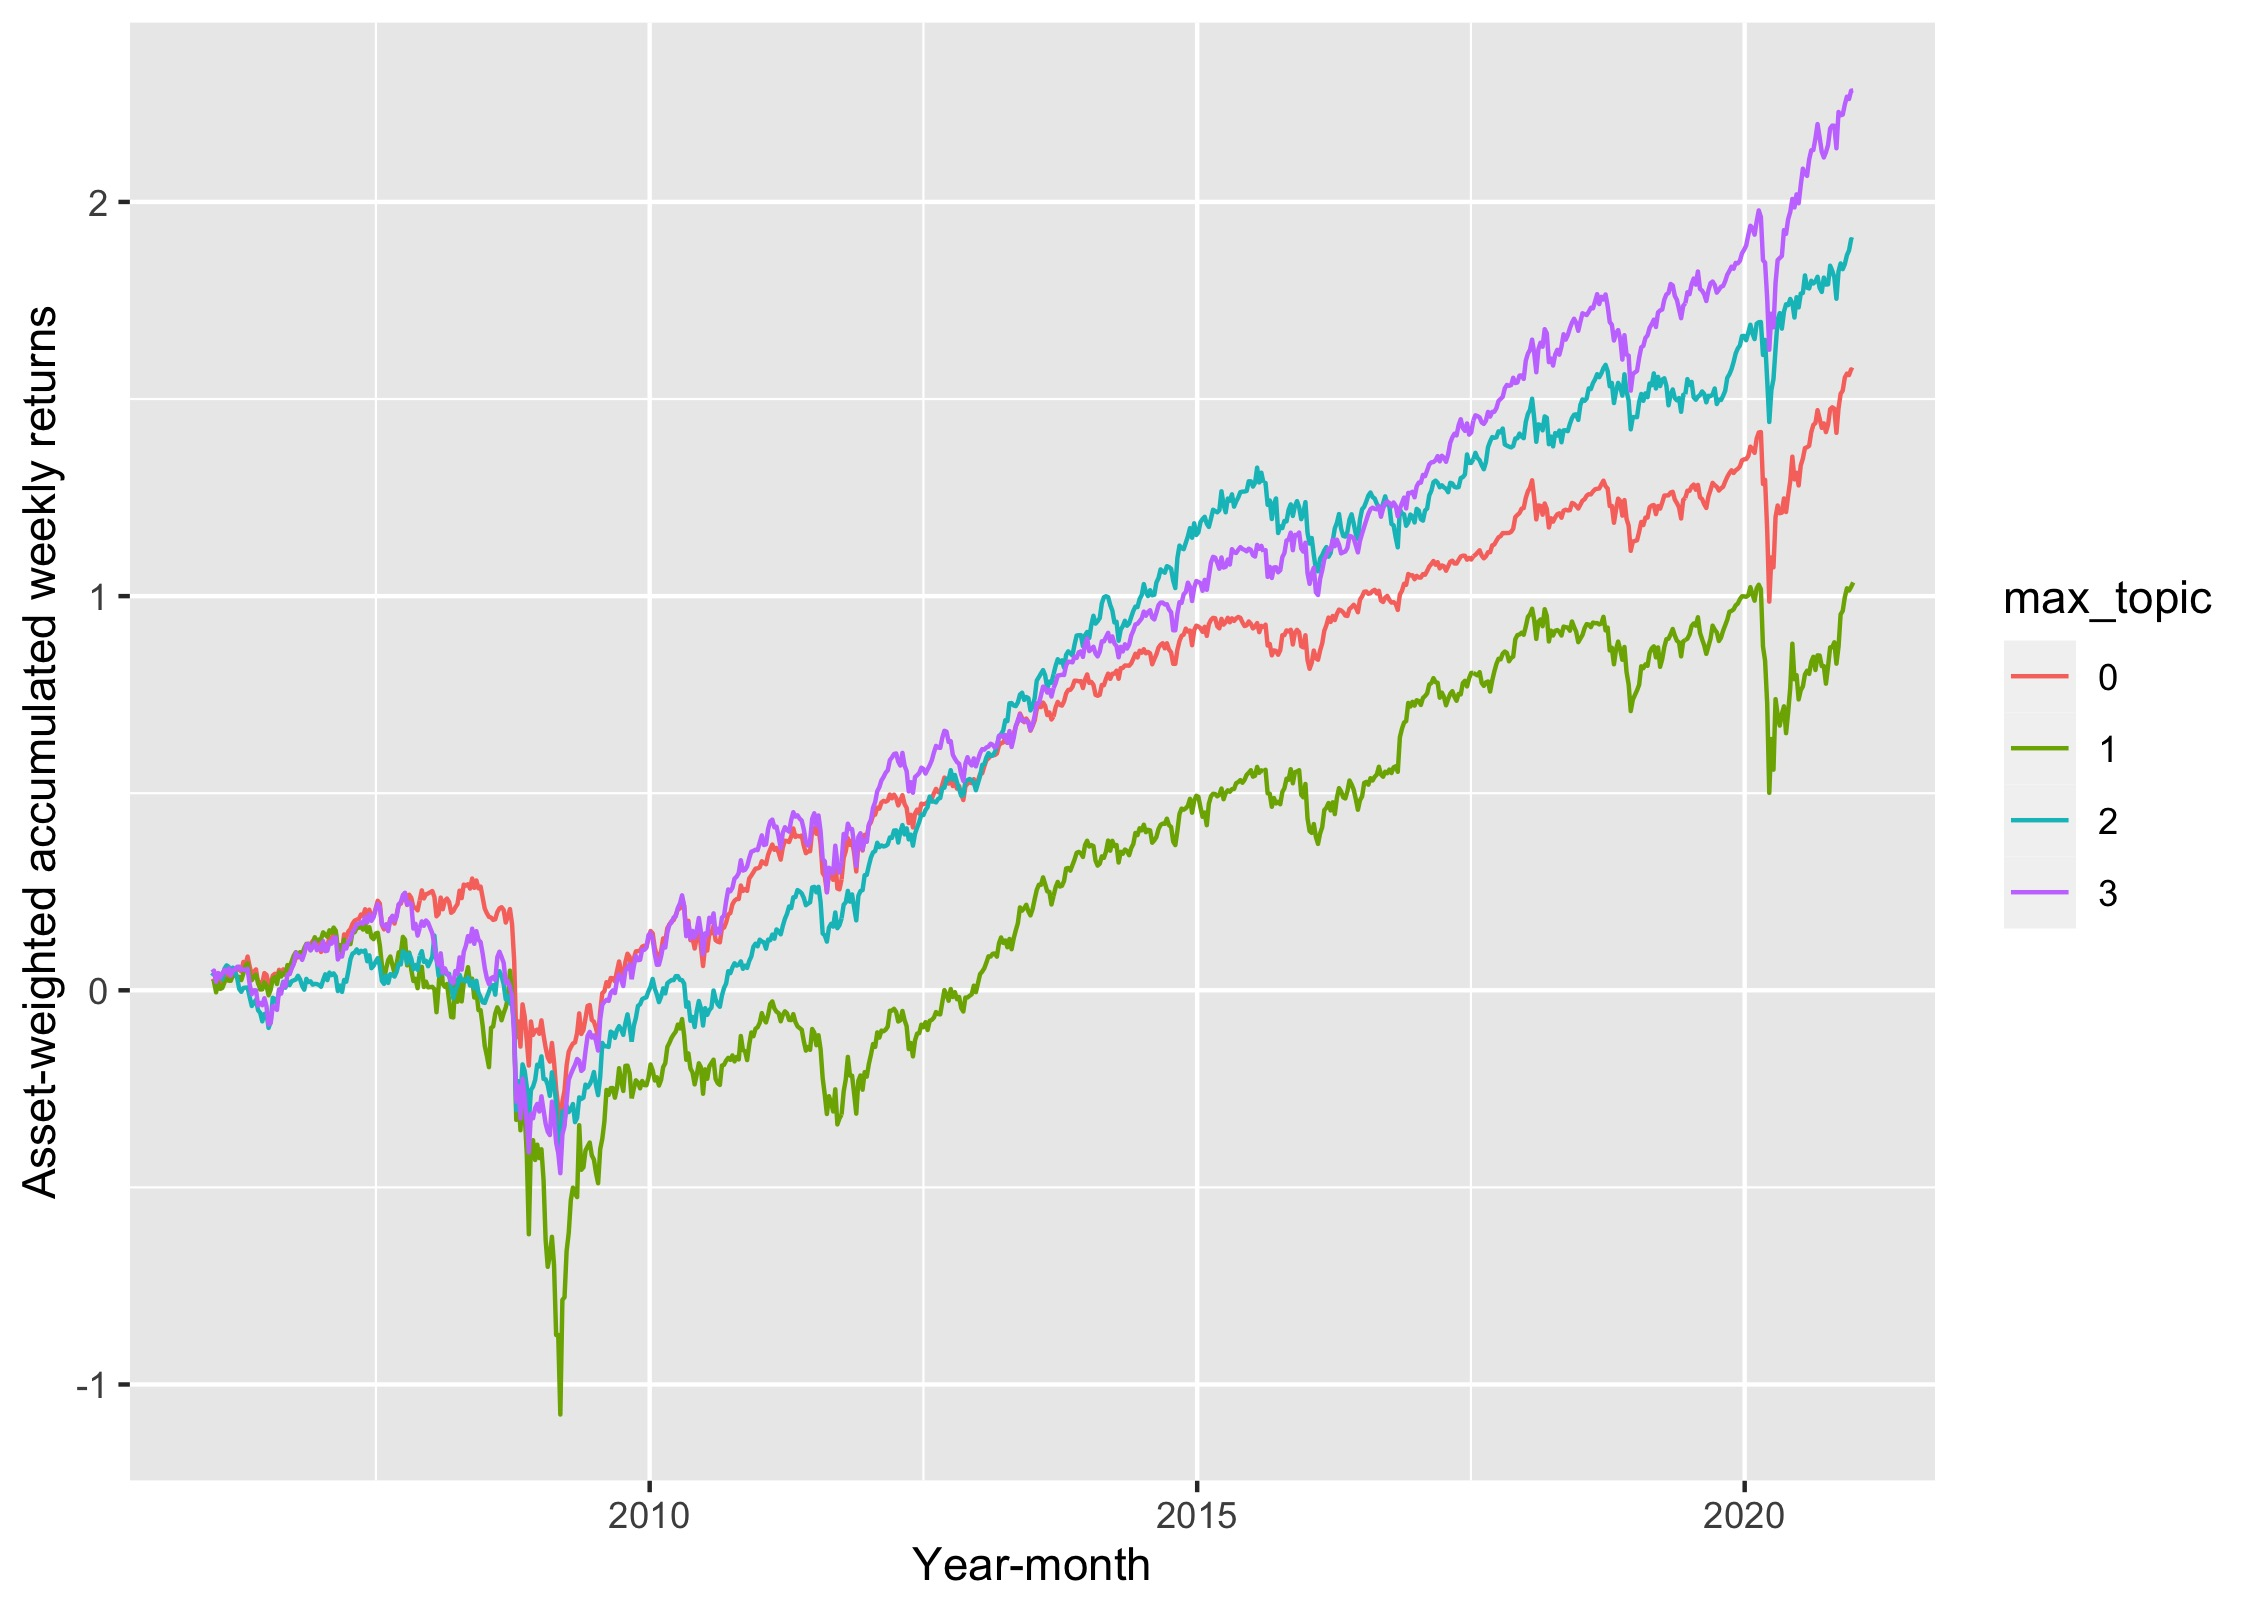
\includegraphics[width=0.6\textwidth]{\ffo/awawr_byg.jpg}
%\FloatBarrier
%
%\insertfigure{stackedplot_at}{Stacked plot of firms' total assets in the upper quartile of KK topic intensity}{0.8}
%
%\insertfigure{stackedplot_n}{-}{0.8}
%
%\insertfigure{topicvsikpt_hm}{-}{0.8}
%
%\insertfigure{topicvskkpt_hm}{-}{0.8}

\bibliography{mylibrary2}

\section*{Appendix A: Text conversion to bag-of-words}

After filtering the firms, I employ the \texttt{spacy} Python library to conduct lemmatization on all the refined texts. Lemmatization transforms words into their base form, ensuring consistent semantics. As an illustration, words such as ``take'', ``took'', and ``taken'' are standardized to ``take''. To do so, \texttt{spacy} leverages WordNet---a comprehensive English lexical database curated by Princeton University.

To extract significant collocations---like ``patent application''---which provide richer semantic insights than individual words, this research adopts the collocation detection method outlined in \cite{Mikolov2013-be}. This methodology yields pertinent bigrams and trigrams. A minimum occurrence threshold of 5 ensures that only the most statistically relevant combinations are incorporated into the dictionary.

This research compiles the entirety of discovered words, bigrams, and trigrams to formulate a dictionary. 

Lastly, the texts are transformed into a bag-of-words model using both the dictionary and the n-gram processed texts. In this representation, each word's frequency in a document, denoted as \(c_{ij}\), is preserved, but the sequence of words is omitted, leading to the final depiction of the corpus.

\begin{figure}[H] % Use [H] to force the figure to be here
  \centering
  \begin{subfigure}{0.45\textwidth}
    \centering
    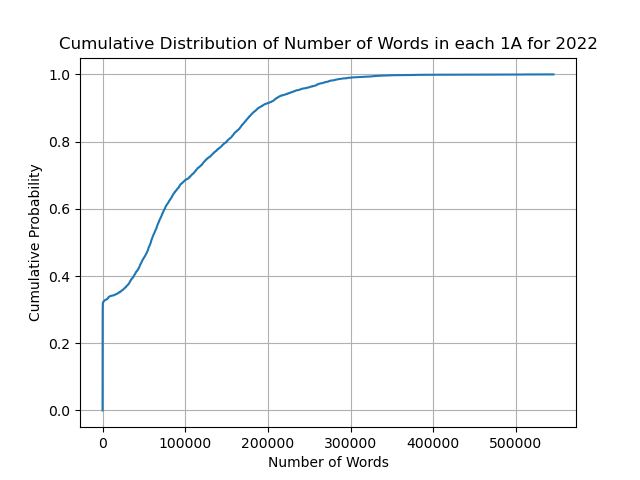
\includegraphics[width=\textwidth]{cdf_words}
	\caption{Cumulative Distribution of Number of Words}	
    \label{fig:figure1}
  \end{subfigure}
  \hfill
  \begin{subfigure}{0.45\textwidth}
    \centering
    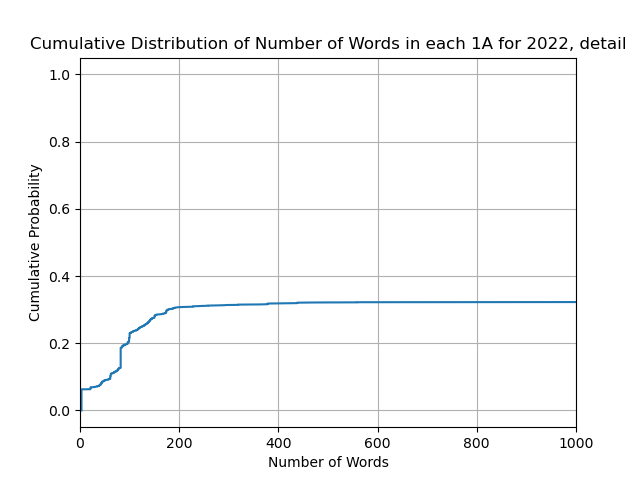
\includegraphics[width=\textwidth]{cdf_words_zoom}
	\caption{Cumulative Distribution of Number of Words, Zoom}
    \label{fig:figure2}
  \end{subfigure}
  \caption{Cumulative Distribution of Number of Words in 2022}
  \label{fig:cdf}
\end{figure}

\insertfigure{stackedplot_at}{Accumulated Assets of Firms in the Upper Quartile of $Topic_{kk}$}{0.8}



\end{document} 